\frame{\frametitle{}
\arenabox{Buying wine}{red!40}{red!10}{
A wine seller has two wine jugs, o small one of 4 liters capacity, and a larger one of 9 liters. 
There is no measuring label mentioned on either of these two jugs i.e. he cannot know the exact amount filled in the jug. 
Can we measure all values from 1 to 9 using these unmarked jugs? (a generalisation of classical water jugs problem)
}

\begin{itemize}
 \item Let \mat{$j_1=4$} be the capacity of the small jug and \mat{$j_2=9$} the capacity of the large jug. 
 \item We use a {\it state space search}, where each state is represented with \mat{$J(x,y)$}: \mat{$x$} is the current amount of wine in jug $j_1$ and 
\mat{$y$} the amount in jug \mat{$j_2$}. 
\item The initial state is \mat{$J(0,0)$}.
\item We use production rules to change the states of the system (\mat{$set(production)$})

 
\end{itemize}
}

\frame{
For the current state \mat{$J(x,y)$}, the following eight actions are possible:

\begin{tabular}{lp{5cm}l}
1. &Fill-in the small jug: & \mat{$J(x,y) \rightarrow J(j_1,y)$}\\
2. &Empty the small jug: &\mat{$J(x,y) \rightarrow J(0,y)$}\\
3. &Fill-in the large jug:& \mat{$J(x,y) \rightarrow J(x,j_2)$}\\
4. &Empty the large jug:& \mat{$J(x,y) \rightarrow J(x,0)$}\\
5. &Empty the small jug into the large jug, if capacity allows this: &
     \mat{$J(x,y) \wedge x+y \leq j_2 \rightarrow J(0,y+x)$}\\
6. &If \mat{$j_2$} does not suffice to empty \mat{$j_1$} then 
 move some amount from the small jug to the larger jug, until \mat{$j_2$} is full:&
 \mat{$J(x,y) \wedge x+y > j_2 \rightarrow J(x -(j_2 -y),j_2)$}  \\  
7. & If capacity of $j_2$ allows, empty the large jug into the small jug:&
     \mat{$J(x,y) \wedge x+y \leq j_1 \rightarrow J(x+y,0)$}\\
8. &If capacity of $j_1$ does not suffice to empty \mat{$j_2$} 
then move some amount from $j_2$, until the $j_1$ is full: & \mat{$J(x,y) \wedge x+y > j_1 \rightarrow J(j_1, y-(j_1 -x))$} \\   
\end{tabular}

\begin{block}{Planning with Prover9}
 \begin{itemize}
  \item Rules are written in clausal form, in order to allow variables in
the \mat{\texttt{\#answer}} directive
\item The\mat{\texttt{\#answer}} directive is useful to print the steps for reaching the
goal.

 \end{itemize}

\end{block}
}

\frame[plain]{
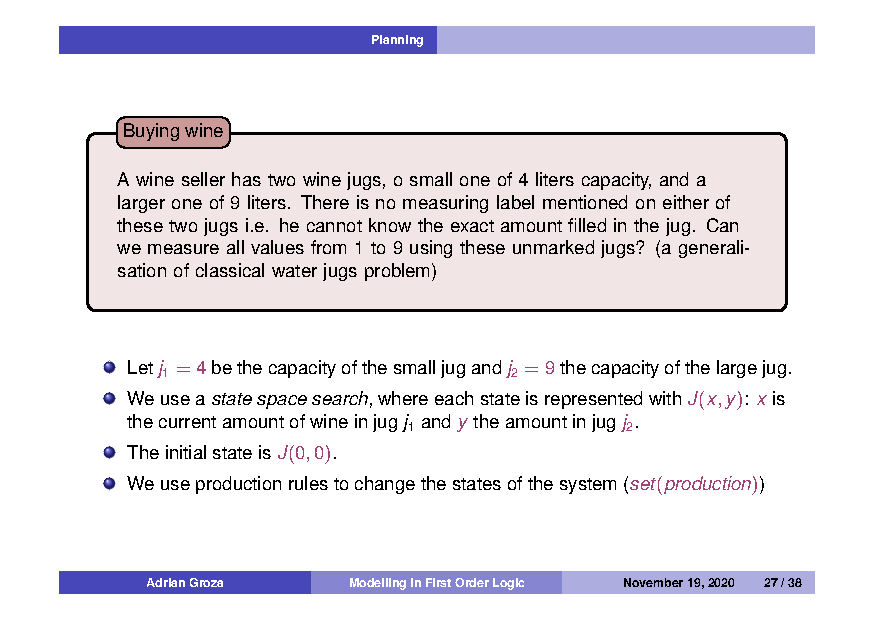
\includegraphics[width=\textwidth]{fig/wine.png}
}

\frame[plain]{\frametitle{Measuring 1 liter of wine \mat{$\exists x\ J(x, 1) \vee \exists y\ J(1,y)$}}
%\centering
\begin{tabular}{l|l|l}
    $Proof_1$ & \#answer(Action)& \#answer(State) \\ \hline
    1 & "init state" & $J(0,0)$\\
    2 & "fill the big jug" & $J(0,j_2)$\\
    3 & "big into small, until full" & $J(j_1,9 -(j_1 -0))$\\
    4 & "empty the small jug" & $J(0,5)$\\
    5 & "big into small, until full" & $J(j_1,5 -(j_1 - 0))$
\end{tabular}
\hspace*{5.5cm}
\vspace*{-1cm}\includegraphics[width=6cm]{fig/liter.png}
}

\frame{\frametitle{Measuring 2 liters of wine}
\mat{$\exists x\ J(x, 2) \vee \exists y\ J(2,y)$}

\begin{center}
\begin{tabular}{r|l|l}
     $Proof_2$ & \#answer(Action)& \#answer(State) \\ \hline
    1 & "init state" & $J(0,0)$\\
    2 & "fill the big jug" & $J(0,j_2)$\\
    3 & "big into small, until full" & $J(j_1,9 -(j_1 - 0))$\\
    4 & "empty the small jug" & $J(0,5)$\\
    5 & "big into small, until full" & $J(j_1,5 -(j_1 - 0))$\\
    6 & "empty the small jug" & $J(0,1)$\\
    7 & "empty the big jug into the small jug" & $J(0 + 1,0)$\\
    8 & "fill the big jug" & $J(1,j_2)$ \\
    9 &  "big into small, until full" & $J(j_1,9 -(j_1 -1))$\\ 
    10 & "empty the small jug" & $J(0,6)$\\
    11 & "big into small, until full" & $J(j_1,6 -(j_1 - 0)))$\\ 
\end{tabular}
\end{center}

%\centering

}

